\documentclass[a4paper]{article}

\usepackage[english]{babel}
\usepackage[utf8]{inputenc}
\usepackage{amsmath}
\usepackage{hyperref}
\usepackage{graphicx}
\usepackage[colorinlistoftodos]{todonotes}

\title{Hologram detection in identity documents - a possible approach}

\author{Alberto Cereser,
    \href{mailto:alberto.cereser@gmail.com}{alberto.cereser@gmail.com} 
}


\date{\today}

\begin{document}
\maketitle

\begin{abstract}
Modern identity documents include anti-fraud holograms. As a first step to detect the holograms, I propose to start with the face pictures and with the features they show at certain angles. The approach presented is general and assumes the presence of holograms on the photo surface. No a priori information on the hologram type is required. 
\end{abstract}

\section{Basic idea}
\label{sec:introduction}

Algorithms are features which are visible only at certain angles, under constant illumination conditions. Different documents are secured using holograms with different shapes and features. The approach I propose is based on the assumption that holograms cover also the face picture(s) in the document. Since comparing {\footnotesize{ID}} images taken at different angles is complicated, I propose to start limiting the analysis to the face pictures only. This is a first step, not a final solution. 

In short, the idea is that the hologram features cannot be considered as face features: they exhibit geometric traits, or contain characters, which can't be find in a human face. 

The approach I propose consists of the following steps:
\begin{itemize}
    \item Detect, in each recorded image, the face images in the document.
    \item Look for non-human traits in the face area. The code should look for edges, curves (e.g., using the Hough transform) and text.
    \item Compare the non-human traits found in different images. The same features should be visible at regular angular intervals as the document is rotated.
\end{itemize}

\section{Example}

I took a video holding my passport and tilting it (see Fig. \ref{fig:pics}). In first approximation, the phone camera is fixed. Then I selected two frames, one where holograms are visible and another where they are not. Following the process outlined in the previous section, I located the face pictures in the document and successfully found some hologram. 

\begin{figure}
    \centering
    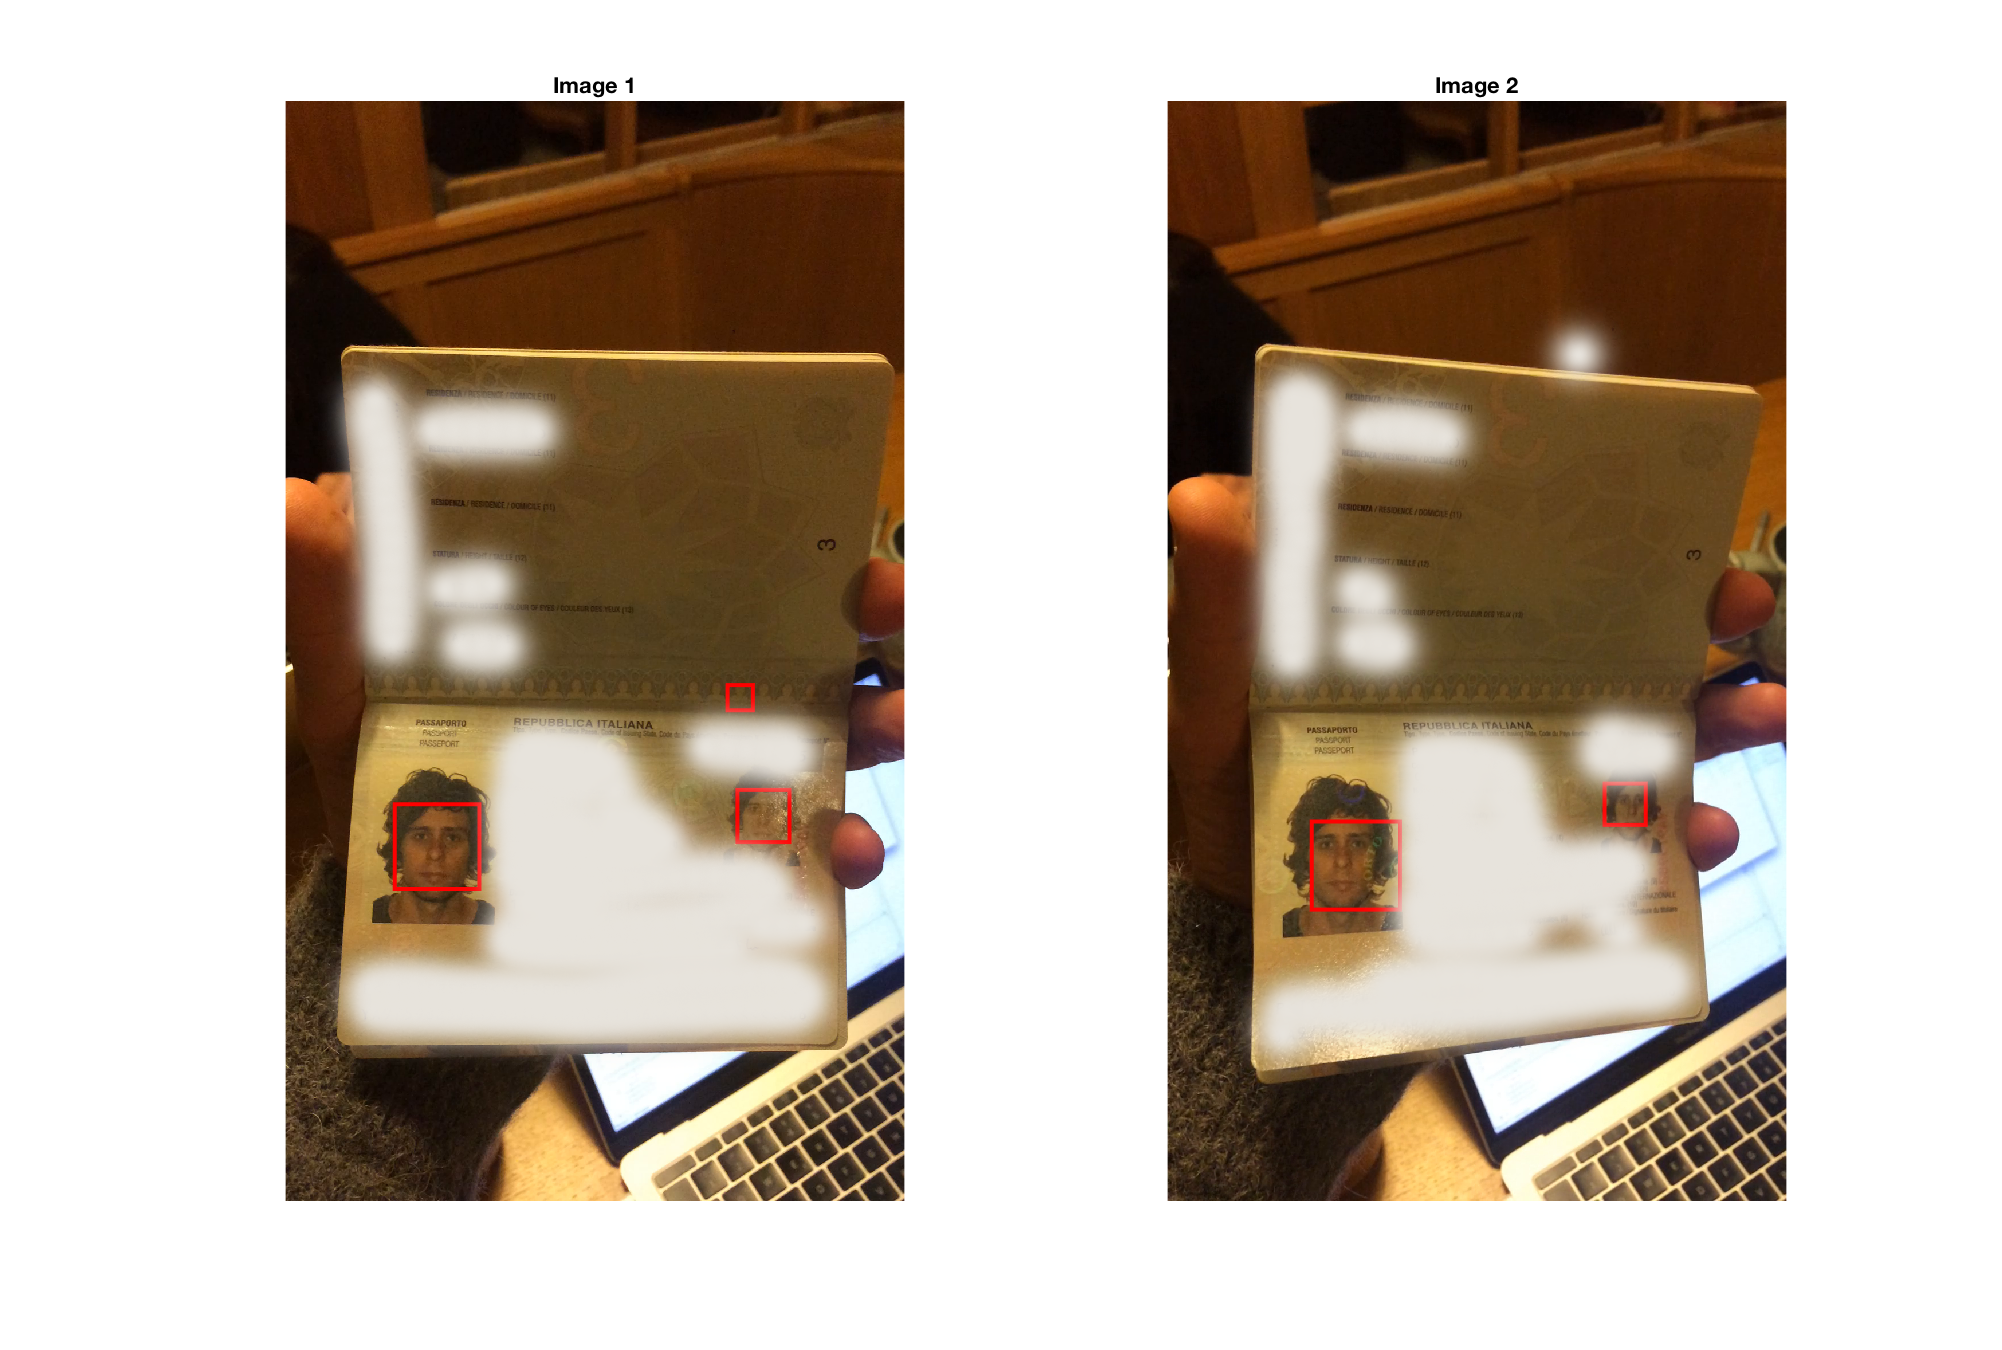
\includegraphics[width=0.8\textwidth]{Angles.png}
    \caption{Two frames from the collected video, recorded at different angles. Face regions are shown in red. The video was collected using an iPhone 5S.}
    \label{fig:pics}
\end{figure}

\begin{figure}[h!]
    \centering
    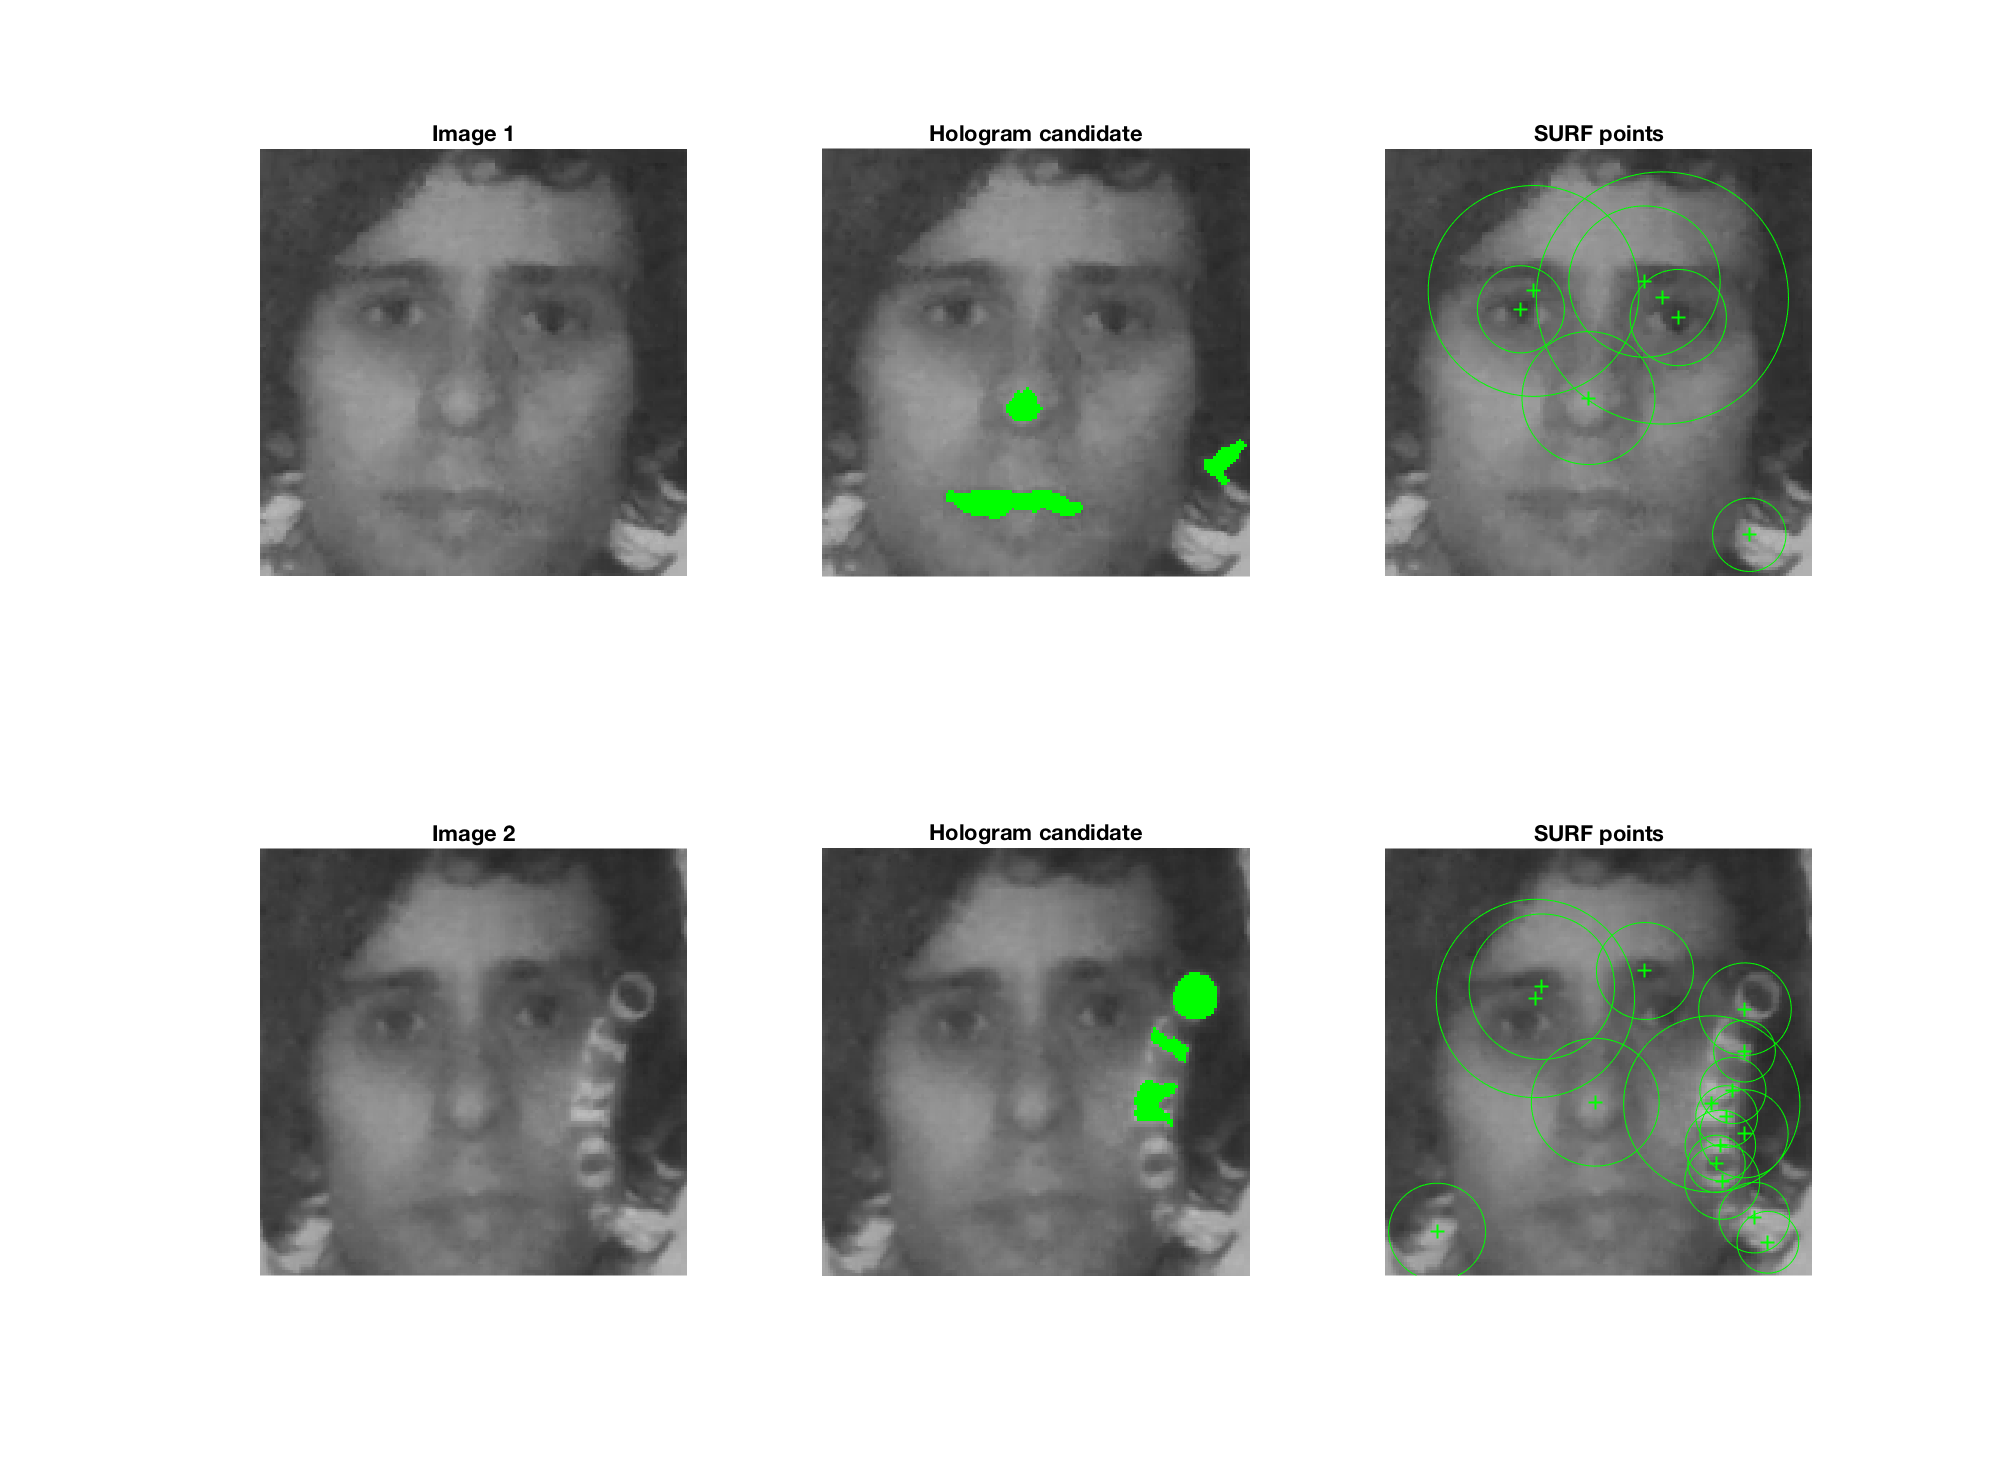
\includegraphics[width=0.9\textwidth]{Detect.png}
    \caption{Overview of the hologram detection algorithm. Holograms show features that are not related to the human physiognomy, such as geometrical shapes (straight or curved lines, ...) and/or text characters. Top: no hologram is present. Bottom: part of the word ``passaporto'' (passport in Italian) can be seen as a hologram. Using  modules already developed, words can be read and their edges can be easily detected.}
    \label{fig:processing}
\end{figure}

\section{Limitations and outlook}

As can be seen in Fig. \ref{fig:processing}, the suggested approach is promising but requires further developments, to avoid false positives detection and to improve text detection (some characters of the hologram are not found, in the figure shown). Steereable filters are promising candidates to enhance characters in the collected images. Solutions to compare holograms collected at different angles need to be implemented

On the other hand, the approach does not rely on a-priori information, and can be extended to detect geometrical shapes. Computationally, analyzing faces is cheaper than analyzing the entire document surface. 

\end{document}